\documentclass[11pt, fleqn]{article}

\usepackage[usenames,dvipsnames,svgnames,table]{xcolor}
\usepackage{amsmath}
\usepackage{amsfonts}
\usepackage[margin=1in]{geometry} % To set the margin widths
\usepackage{graphicx}
\usepackage{listings}
\usepackage{multirow}
\usepackage{tabularx}
\usepackage{varioref}
\usepackage[noabbrev,capitalize]{cleveref}
\usepackage[group-separator={,}]{siunitx}
\usepackage{subcaption}
\usepackage{titlesec}
\usepackage{lscape}
\usepackage{bm}
\usepackage[titletoc,toc,title]{appendix}

\lstset{
  frame=single,
  basicstyle=\ttfamily,% print whole listing small
  language=R,
  aboveskip=3mm,
  belowskip=3mm,
  showstringspaces=false,
  columns=flexible,
  numbers=none,
  commentstyle=\color{ForestGreen},
  stringstyle=\color{Maroon},
  breaklines=true,
  breakatwhitespace=true,
  tabsize=2,
  literate={<-}{{$\gets$}}1 {~}{{$\sim$}}1
}

\sisetup{output-exponent-marker=\textsc{e}}

\setlength{\parskip}{12pt} % Sets a blank line in between paragraphs
\setlength\parindent{0pt} % Sets the indent for each paragraph to zero

\begin{document}

\title{Machine Learning (41204-01)\\HW \#7}
\author{Will Clark and Matthew DeLio \\
\textsf{\{will.clark,mdelio\}@chicagobooth.edu} \\
University of Chicago Booth School of Business}
\date{\today}
\maketitle

\section{Zachary's Karate Club}

Zachary's Karate Club is a network describing a university karate club from the early 1970's. The network has 34 vertices and 78 edges as depicted in \cref{fig:karate_network}. The network was observed and described by Wayne W. Zachary during and after it split into two factions (led by John A and Mr. Hi, denoted with blue circles and red squares, respectively). Because we know the features of the network and the factions into which it split, it is an ideal data set on which to test out various community detection algorithms.

\begin{figure}[!htb]
\centering
\caption{Zachary's Karate Club and Factions}
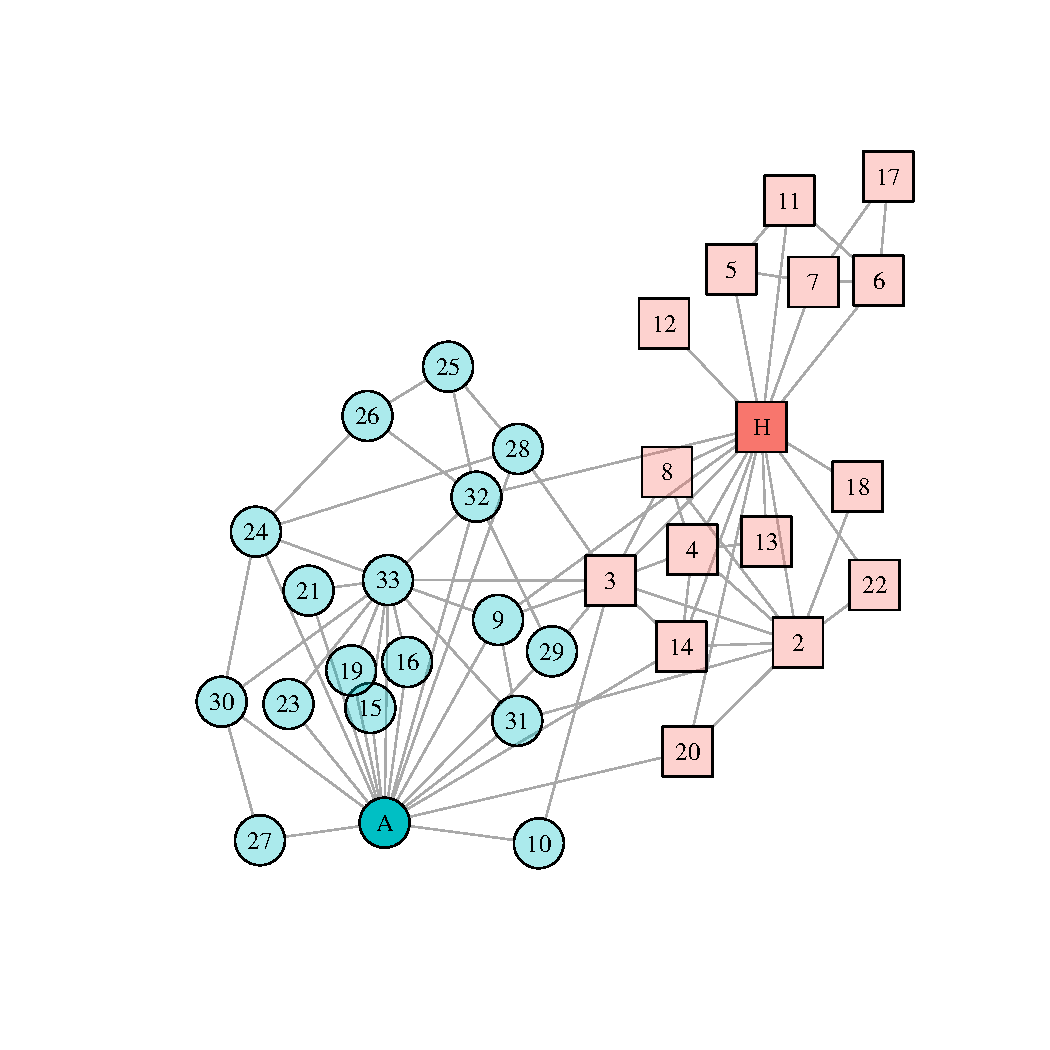
\includegraphics[scale=.5,trim={0.75in 0.75in 0.75in 0.75in}, clip=True]{karate_network.pdf}
\label{fig:karate_network}
\end{figure}

We used the algorithms listed below to try and determine the underlying community structure in Zachary's karate club. The results are visualized in \cref{fig:edge_betweenness}-\cref{fig:walktrap}. The hierarchical algorithm can be cut into two groups and compared directly to the ground truth of the observed factions, but algorithms with more groups are tougher to evaluate. If an algorithm produces more than two groups, as long as the groups are contained entirely within one faction or the other, we consider there to be no mis-classifications. In the associated figures, members of Mr. H's faction are in squares and members of John A's faction are in circles; the colors are set according to algorithmically-determined groups.
\begin{itemize}
\item \textbf{Edge Betweenness}: A hierarchical algorithm that we cut to obtain two groups. The default setting is for the algorithm to consider the network edge weights, but in doing so the algorithm misclassifies two vertices (Actors 3 and 14; see \cref{fig:edge_betweenness}). By ignoring the edge weights, the algorithm only mis-classifies one vertex (Actor 3). 
\item \textbf{Greedy Modularity Optimization (Fast Greedy)}: A hierarchical algorithm that we cut to obtain two groups. It correctly predicts the faction for all vertices (see \cref{fig:fast_greedy}).
\item \textbf{Infomap}: A non-hierarchical algorithm that splits the data into 3 groups. Two groups are made entirely of members from Mr. Hi's faction (see \cref{fig:infomap}).
\item \textbf{Propagating Labels}: A non-hierarchical algorithm that splits the data into 3 groups. Two groups are made entirely of members from Mr. Hi's faction. It classifies the networks into the same groups as the Infomap algorithm (see \cref{fig:label_prop}).  
\item \textbf{Leading Eigenvector}: This is another hierarchical algorithm, although the basic \textsf{cutat} function produces an error when we attempt to break the network into two communities.\footnote{\textsf{Warning message: In cutat(cl, 2) : Cannot have that few communities}} As an alternative, we visualize the network as a dendrogram and use the two largest branches as our estimate of the factions. The restuls are not good; five actors in each group are mis-categorized. The results are in \cref{fig:leading_eigen}. This is far and away the worst algorithm for this data set, although it may be because of the implementation in \textsf{igraph}.
\item \textbf{Multi-level Modularity Optimization (Louvain)}: A non-hierarchical algorithm that splits the data into 4 groups. Two groups are made entirely of members from Mr. Hi's faction and two groups are made entirely of members from John A's faction. This algorithm breaks Mr. Hi's faction into the same groups that the Infomap and Propagating Labels algorithms do (see \cref{fig:louvain}).
\item \textbf{Optimal Structure}: A non-hierarchical algorithm that splits the data into 4 groups. The four groups are identical to those identified by the Multi-Level Modularity Optimization algorithm above (see \cref{fig:optimal}).
\item \textbf{Statistical Mechanics (Spinglass)}: A non-hierarchical algorithm that splits the data into 4 groups. The groups are nearly the same as those identified in the Optimal Structure and Multi-Level Modularity Optimation algorithms, except Actor 24 has switched groups within John A's faction (see \cref{fig:spinglass}).
\item \textbf{Short Random Walks (Walktrap)}: A hierarchical algorithm that we cut to obtain two groups. It correctly predicts the faction for all vertices (see \cref{fig:walktrap}).
\end{itemize}
Ultimately, all algorithms besides the Edge Betweenness and Leading Eigenvector algorithm correctly break the network into the correct groups, either the observed factions or subsets of the observed factions.

%%%%%%%%%%%%%%%%%%%% KARATE COMMUNITY GRAPHS %%%%%%%%%%%%%%%%%%%%
\begin{figure}
\centering
\begin{subfigure}[b]{0.32\textwidth}
\caption{Edge Betweenness}
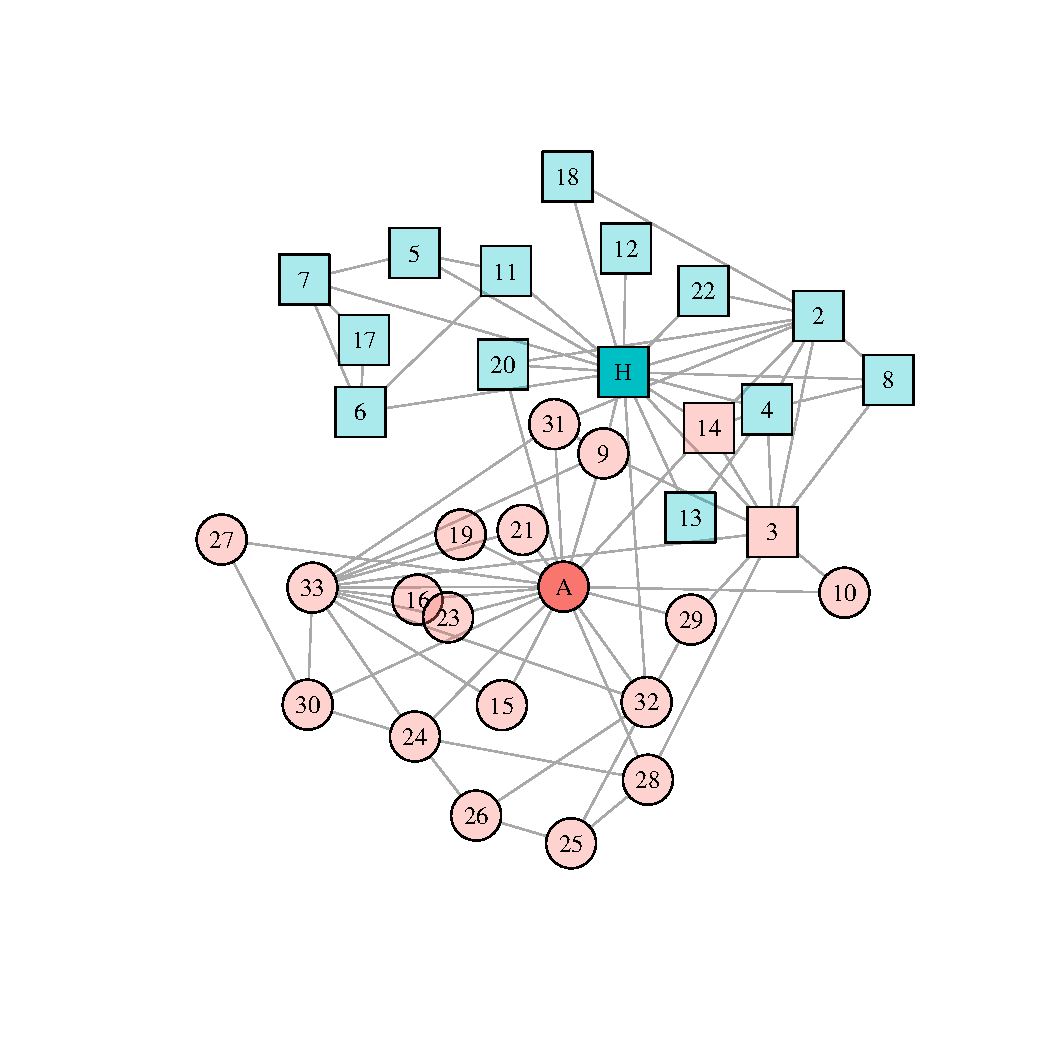
\includegraphics[width=\textwidth,trim={0.75in 0.75in 0.75in 0.75in}, clip=True]{edge_betweenness.pdf}
\label{fig:edge_betweenness}
\end{subfigure}
\hfill
\begin{subfigure}[b]{0.32\textwidth}
\caption{Greedy Optimization}
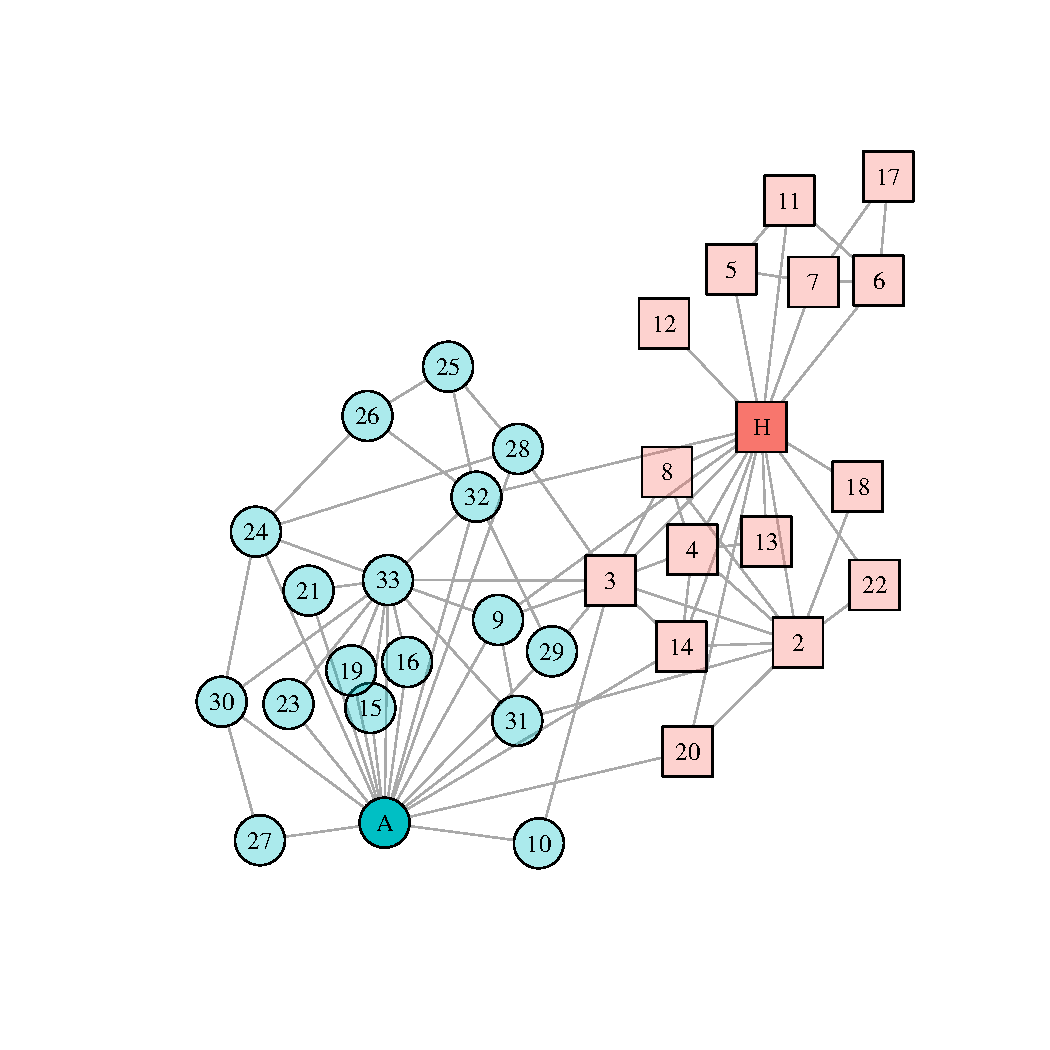
\includegraphics[width=\textwidth,trim={0.75in 0.75in 0.75in 0.75in}, clip=True]{fast_greedy.pdf}
\label{fig:fast_greedy}
\end{subfigure}
\hfill
\begin{subfigure}[b]{0.32\textwidth}
\caption{Infomap}
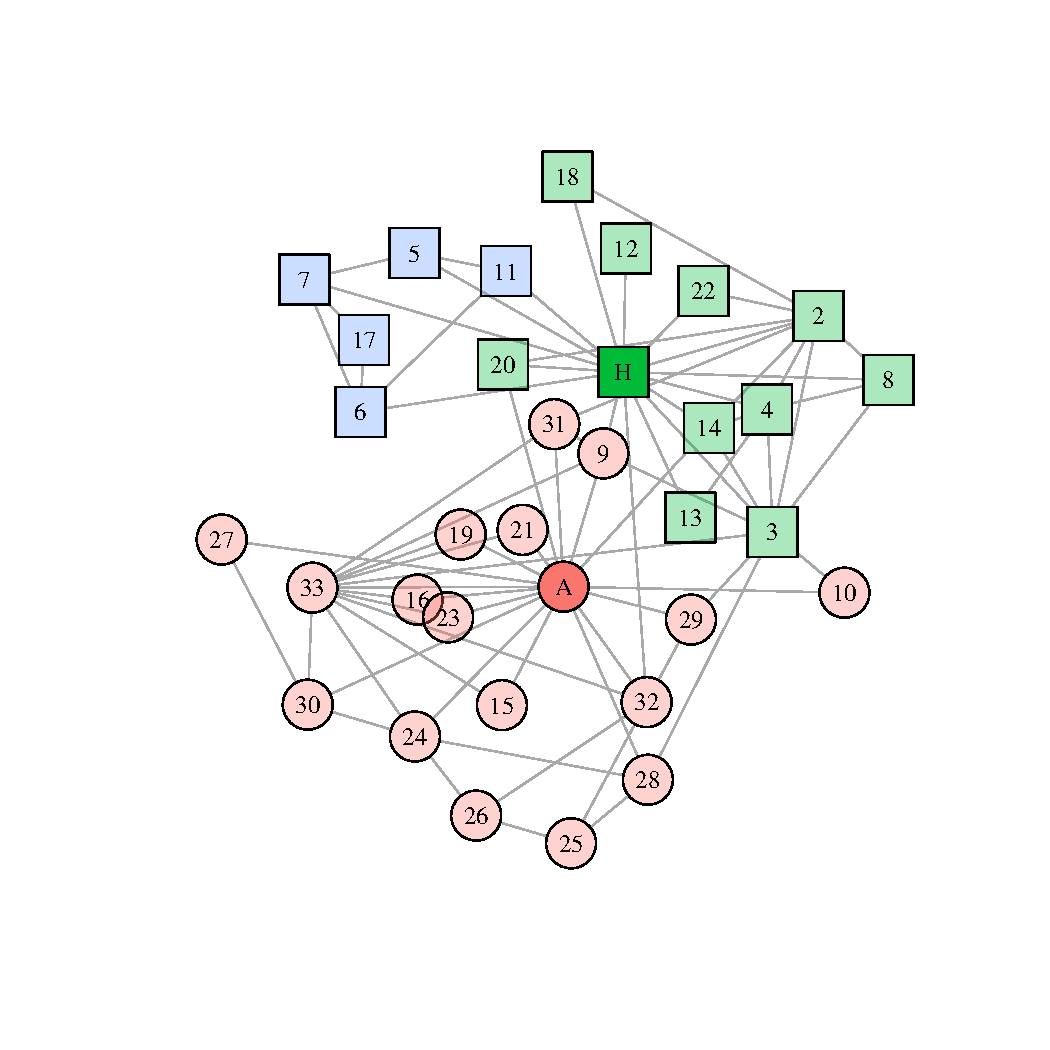
\includegraphics[width=\textwidth,trim={0.75in 0.75in 0.75in 0.75in}, clip=True]{infomap.pdf}
\label{fig:infomap}
\end{subfigure}

\begin{subfigure}[b]{0.32\textwidth}
\caption{Propagating Labels}
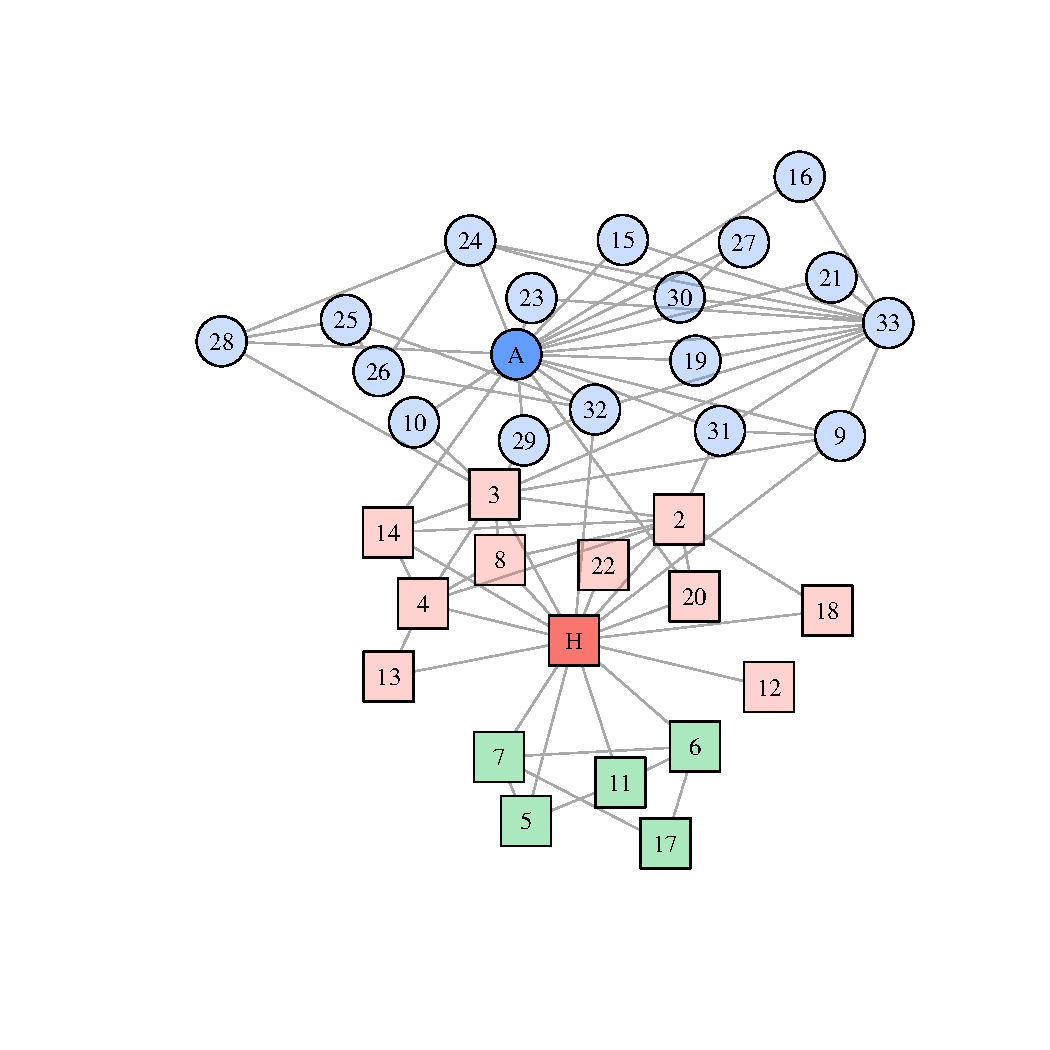
\includegraphics[width=\textwidth,trim={0.75in 0.75in 0.75in 0.75in}, clip=True]{label_prop.pdf}
\label{fig:label_prop}
\end{subfigure}
\hfill
\begin{subfigure}[b]{0.32\textwidth}
\caption{Leading Eigenvector}
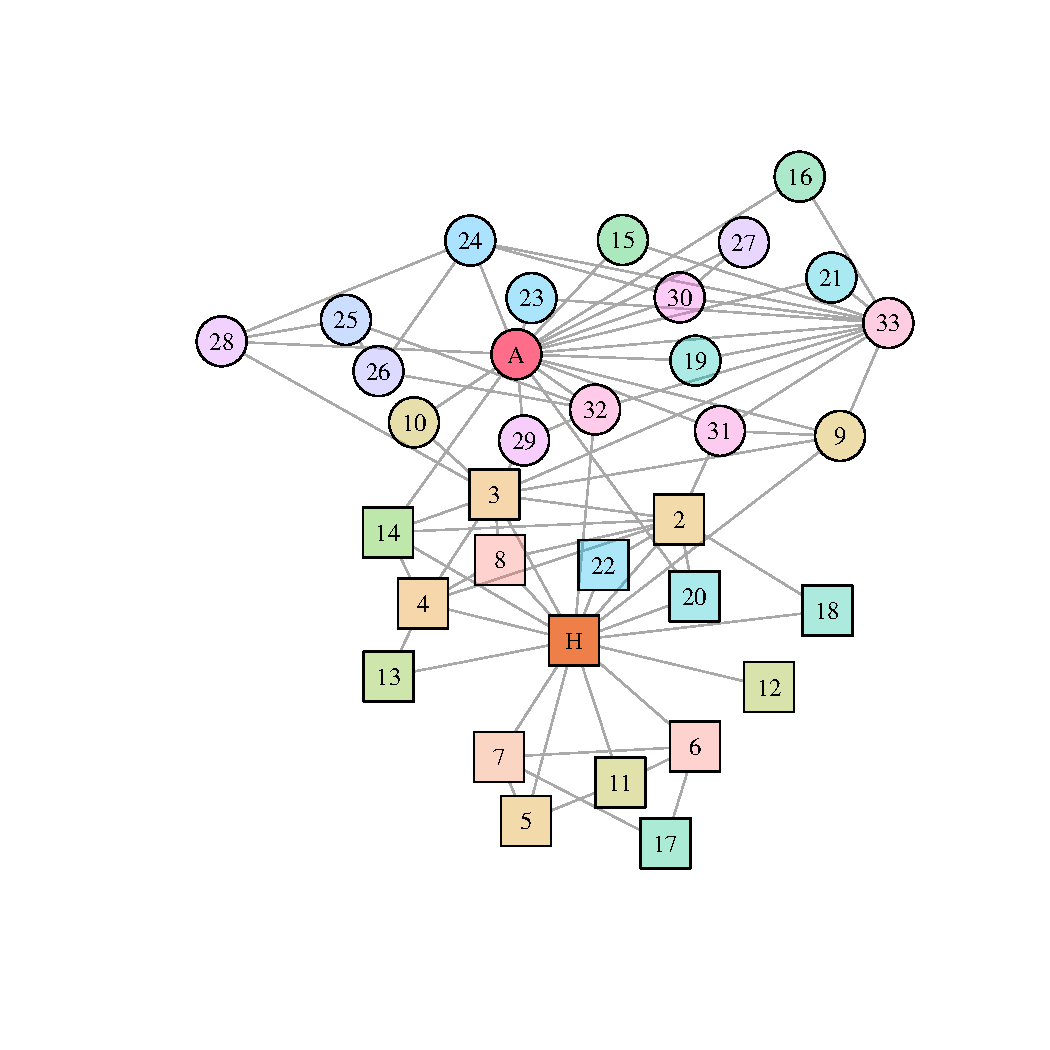
\includegraphics[width=\textwidth,trim={0.75in 0.75in 0.75in 0.75in}, clip=True]{leading_eigen.pdf}
\label{fig:leading_eigen}
\end{subfigure}
\hfill
\begin{subfigure}[b]{0.32\textwidth}
\caption{Multi-level Optimization}
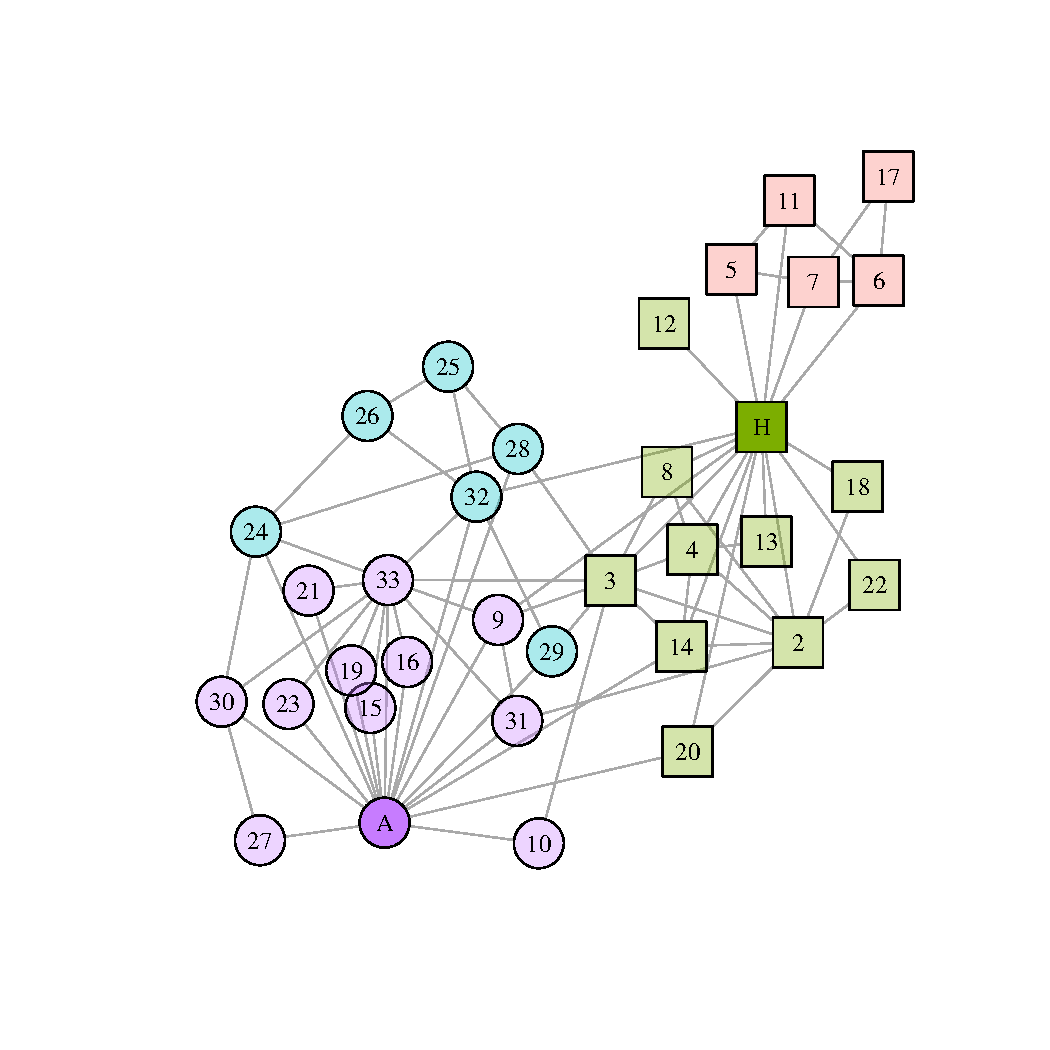
\includegraphics[width=\textwidth,trim={0.75in 0.75in 0.75in 0.75in}, clip=True]{louvain.pdf}
\label{fig:louvain}
\end{subfigure}

\begin{subfigure}[b]{0.32\textwidth}
\caption{Optimal Structure}
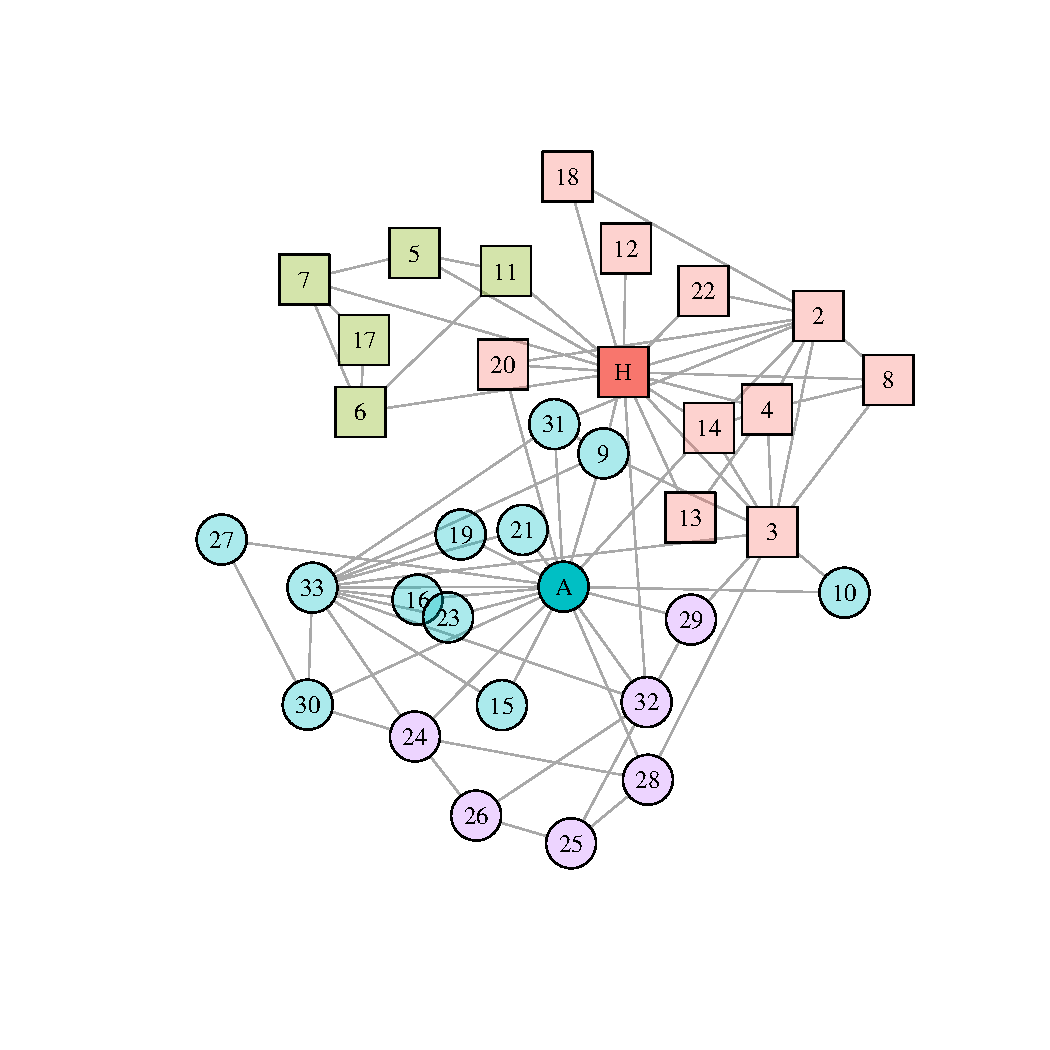
\includegraphics[width=\textwidth,trim={0.75in 0.75in 0.75in 0.75in}, clip=True]{optimal.pdf}
\label{fig:optimal}
\end{subfigure}
\hfill
\begin{subfigure}[b]{0.32\textwidth}
\caption{Statistical Mechanics}
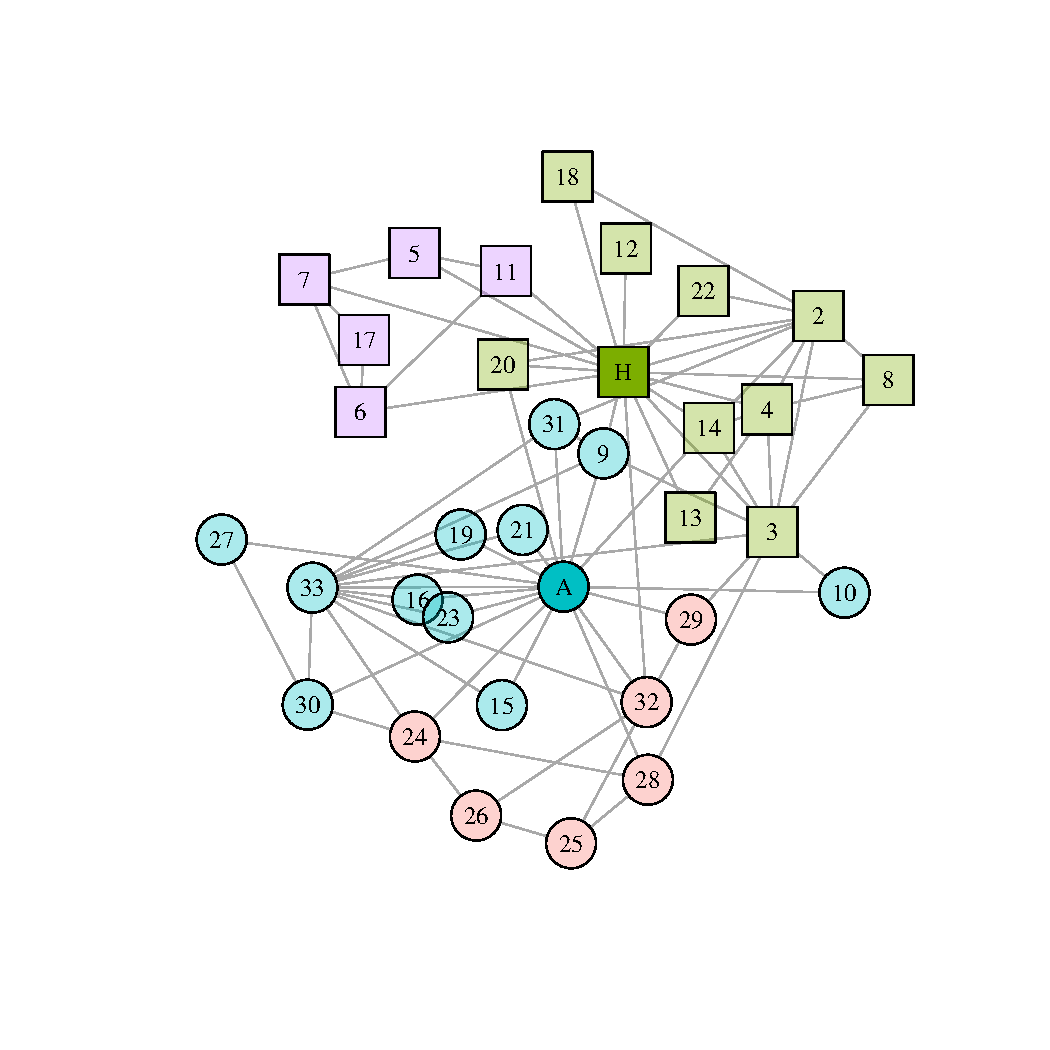
\includegraphics[width=\textwidth,trim={0.75in 0.75in 0.75in 0.75in}, clip=True]{spinglass.pdf}
\label{fig:spinglass}
\end{subfigure}
\hfill
\begin{subfigure}[b]{0.32\textwidth}
\caption{Short Random Walks}
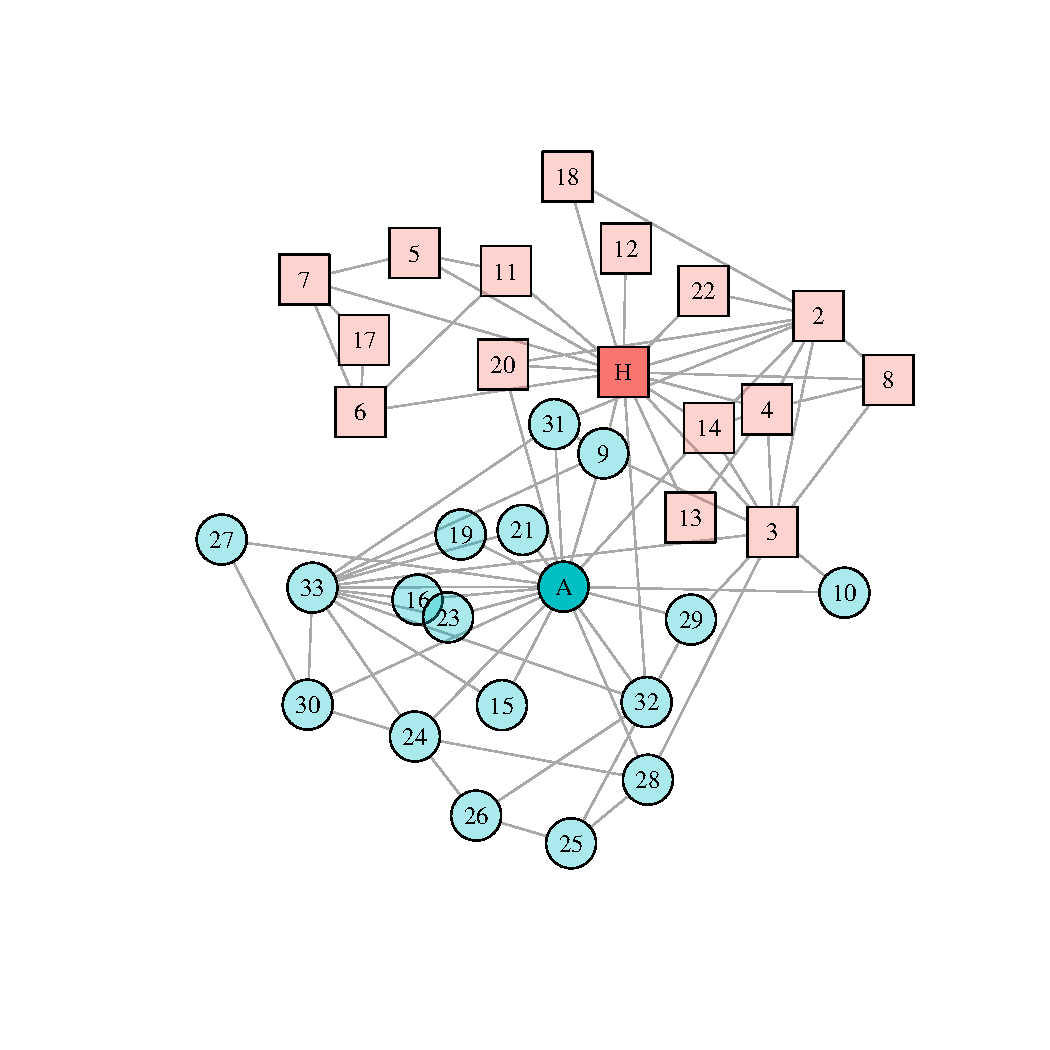
\includegraphics[width=\textwidth,trim={0.75in 0.75in 0.75in 0.75in}, clip=True]{walktrap.pdf}
\label{fig:walktrap}
\end{subfigure}
\caption{Community Detection Algorithms for Zachary's Karate Club}
\end{figure}
%%%%%%%%%%%%%%%%%%%%%%%%%%%%%%%%%%%%%%%%%%%%%%%%%%%%%%%%%%%%%%%%%

\section{Wikipedia}
\subsection{Clustering}
Due to the size of the data-set, we apply at the first clustering algorithm that we got working on the data.

\begin{figure}
  \centering
  \begin{subfigure}[b]{0.49\textwidth}
    \caption{Cluster-Size}
    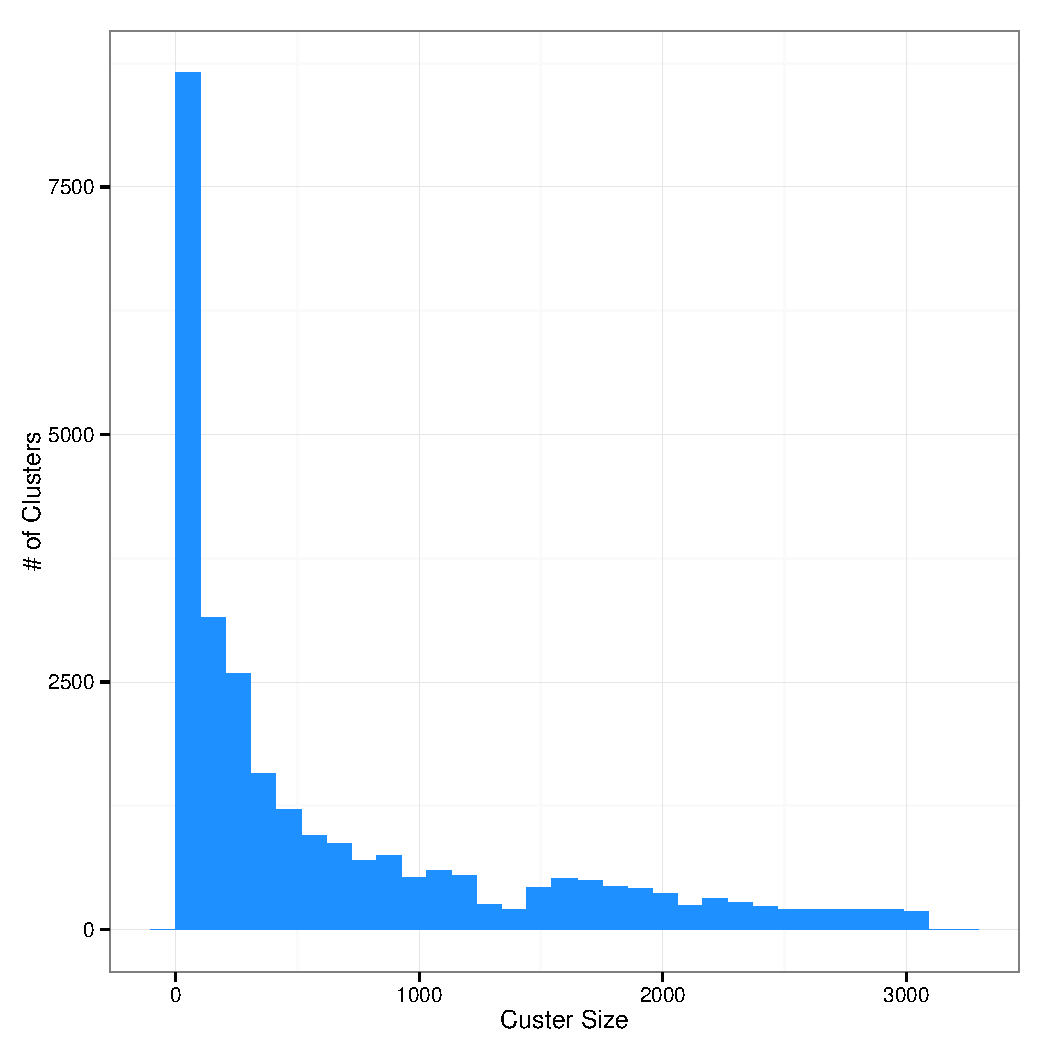
\includegraphics[width=\textwidth]{wiki_cl_hist.pdf}
    \label{fig:wiki_size}
  \end{subfigure}
  \hfill
  \begin{subfigure}[b]{0.49\textwidth}
    \caption{Vertex Connectedness}
    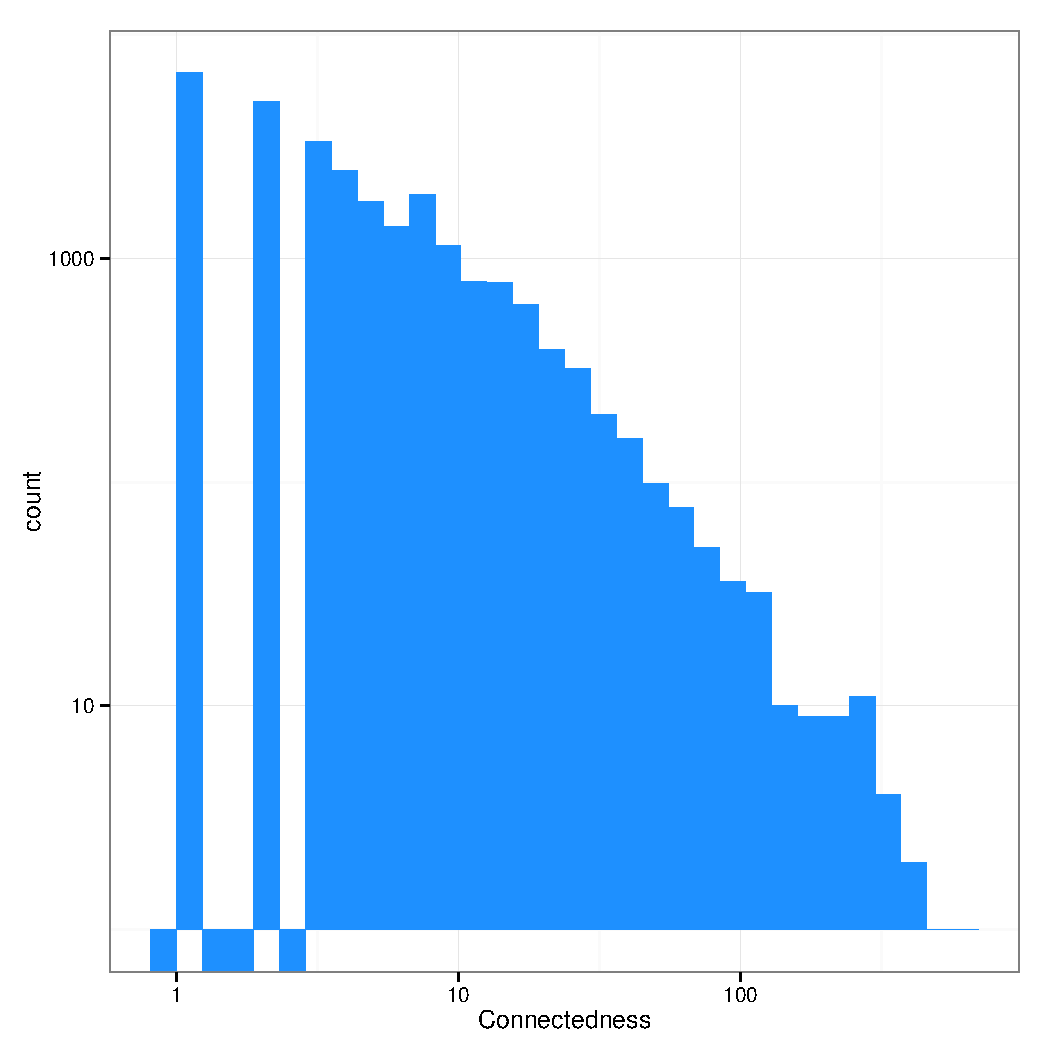
\includegraphics[width=\textwidth]{wiki_edge_hist.pdf}
    \label{fig:wiki_conn}
  \end{subfigure}
  \caption{}
\end{figure}

% \begin{figure}[!htb]
%   \centering
%   \caption{Visual Representation of the Largest 8 Clusters}
%   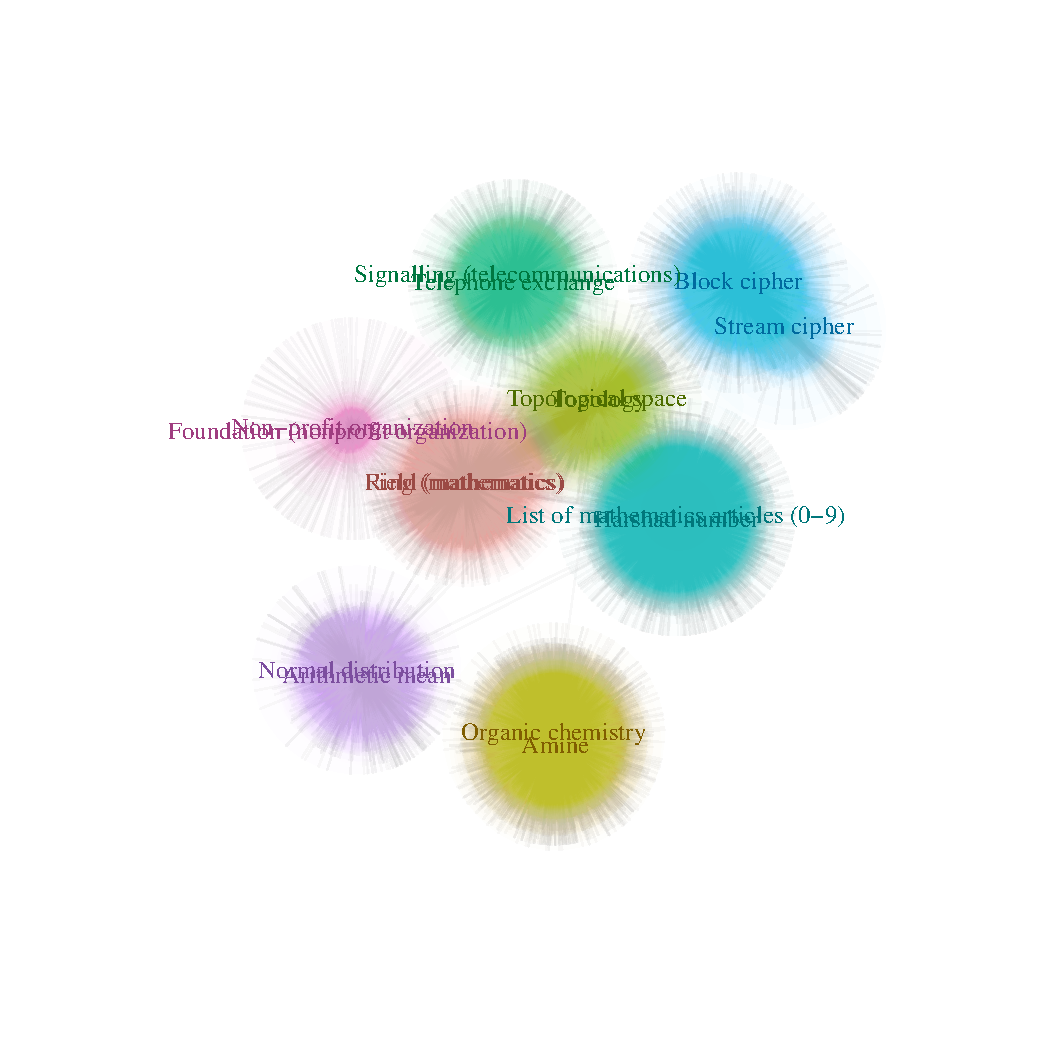
\includegraphics[width=\textwidth]{wiki_clust.pdf}
%   \label{fig:wiki_clust}
% \end{figure}

\begin{landscape}
% latex table generated in R 3.2.2 by xtable 1.8-0 package
% Thu Nov 19 13:05:13 2015
\begin{table}[ht]
\centering
\caption{Sample Topics for 4 Largest Clusters} 
\label{tab:wiki_topics}
\begin{tabular}{llll}
  \hline
1 & 2 & 3 & 6 \\ 
  \hline
Finitely-generated module & Electrophilic halogenation & Train track & Proceed-to-select \\ 
  SINGULAR & Butyl & Fréchet space & N11 code \\ 
  Jordan-Chevalley decomposition & Aromatic compound & Luzin space & Kewlstart \\ 
  Ring extension & Azirines & Uniform property & Ringer equivalence number \\ 
  Indecomposable module & Wieland-Miescher ketone & Dual topology & Attendant console \\ 
  Ideal quotient & Phenylene & Continuous function (topology) & Long-haul communications \\ 
  Maximal ideal & Cyclosilane & Opial property & Skip (radio) \\ 
  Brahmagupta&apos;s problem & Ketone halogenation & Positive element & Dial tone \\ 
  Separable extension & Methylene shuffle & Sigma-compact space & Intercharacter interval \\ 
  Complete algebraic variety & Phthalimide & Operator topology & Night service \\ 
   \hline
\end{tabular}
\end{table}

\end{landscape}


\begin{appendices}

\end{appendices}

\end{document}

% \input{.tex}

% \begin{figure}
%   \centering
%   \begin{subfigure}[b]{0.49\textwidth}
%     \caption{}
%     \includegraphics[width=\textwidth]{.pdf}
%     \label{fig:}
%   \end{subfigure}
%   \hfill
%   \begin{subfigure}[b]{0.49\textwidth}
%     \caption{}
%     \includegraphics[width=\textwidth]{.pdf}
%     \label{fig:}
%   \end{subfigure}
%   \caption{}
% \end{figure}

% \begin{figure}[!htb]
%   \centering
%   \caption{}
%   \includegraphics[scale=.5]{.pdf}
%   \label{fig:}
% \end{figure}

